% DDPG vs DPG comparison. (The earlier fragile pixel-positioned red boxes and
% the DDPG/DPG header labels+arrows have been removed; the column groups are
% explained in the side text instead.)

% Slide: results table with side explanation
\begin{frame}{Experiments --- Is DDPG better than DPG?}
\begin{columns}[c]
\begin{column}{0.24\textwidth}
\footnotesize
Normalised return (1.0 $\approx$ planning baseline) across 30+ tasks.
\\[0.6em]
\textbf{DDPG} columns: low-dim (\emph{lowd}) and pixel (\emph{pix}) inputs.
\\[0.4em]
\textbf{DPG} columns: original control (\emph{cntrl}).
\end{column}
\begin{column}{0.76\textwidth}
\centering
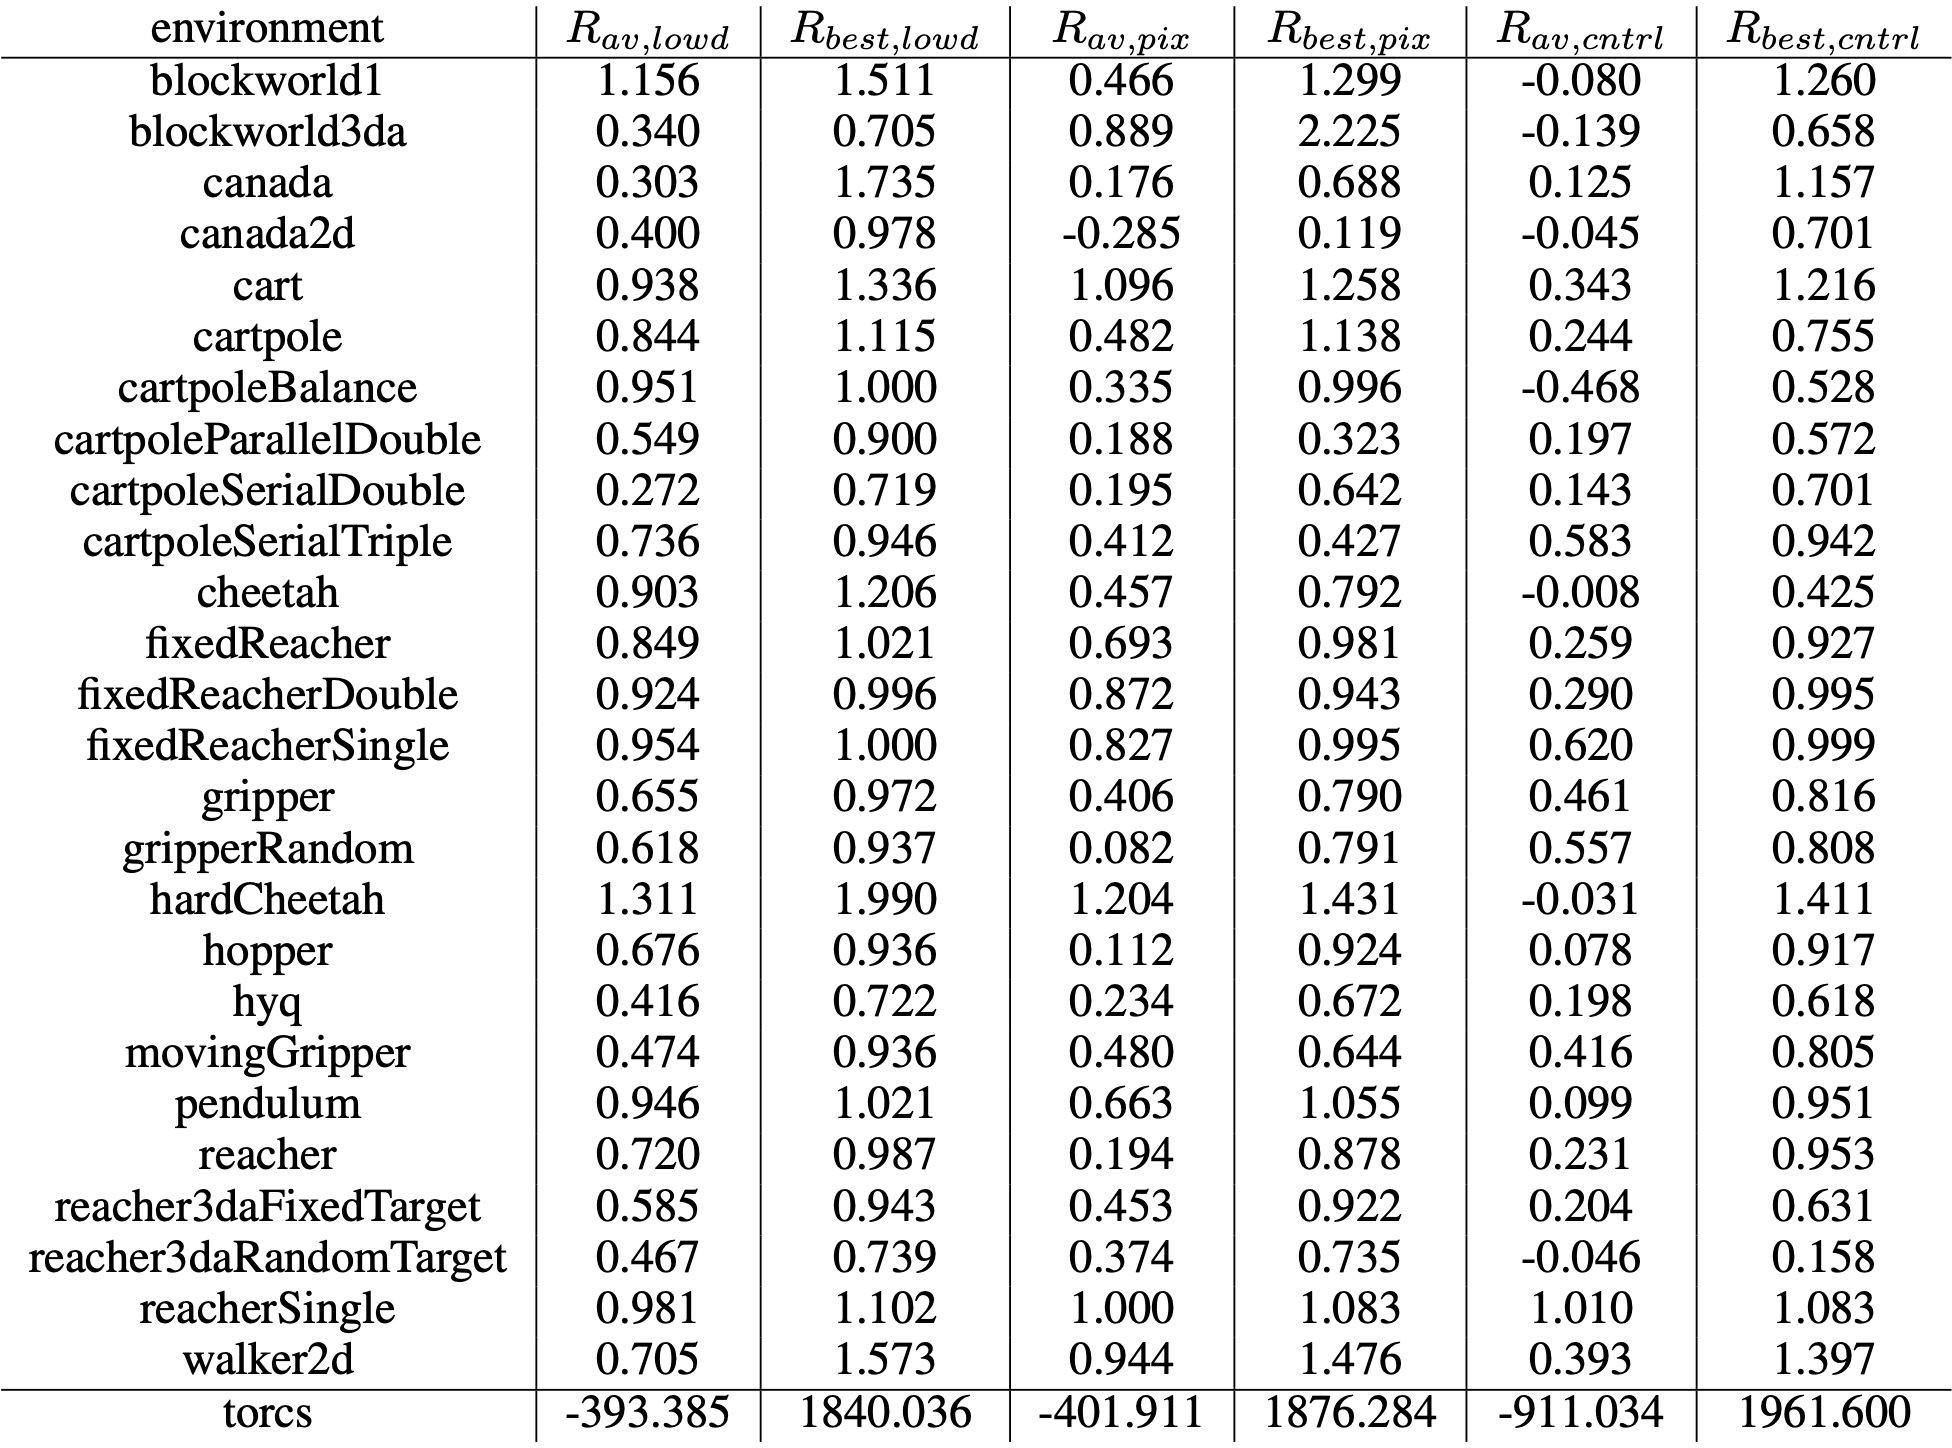
\includegraphics[width=\linewidth,height=0.78\textheight,keepaspectratio]{images/continuous-control-1/figures/ddpg-vs-dpg-table.jpg}
\end{column}
\end{columns}
\begin{flushright}\tiny Table: DDPG \rref{5}\end{flushright}
\end{frame}

% Slide: the high-variance takeaway, made with a clean native excerpt table
% (no fragile image overlays).
\begin{frame}{Experiments --- DDPG still exhibits high variance}
\vspace{0.3em}
DDPG often reaches a strong \emph{best} run, but its \emph{average} return is far lower --- a large gap signals instability across seeds/episodes:
\vspace{0.6em}
\begin{center}
\renewcommand{\arraystretch}{1.3}
\small
\begin{tabular}{lcc}
\hline
\textbf{Environment} & $\boldsymbol{R_{av,\,lowd}}$ & $\boldsymbol{R_{best,\,lowd}}$ \\
\hline
cart      & 0.938   & 1.336 \\
pendulum  & 0.946   & 1.021 \\
canada    & \textcolor{red}{0.303}   & 1.735 \\
gripper   & \textcolor{red}{0.618}   & 0.972 \\
torcs     & \textcolor{red}{$-393.4$} & 1840.0 \\
\hline
\end{tabular}
\end{center}
\vspace{0.5em}
\footnotesize
\begin{itemize}
    \item Simple tasks (cart, pendulum): average $\approx$ best --- stable.
    \item Harder tasks (canada, gripper) and especially \textbf{torcs}: average collapses while best stays high $\Rightarrow$ \textcolor{red}{\textbf{high variance / brittleness}}.
    \item This overestimation-driven instability is exactly what \textbf{TD3} later targets.
\end{itemize}
\end{frame}
